% !TEX encoding = UTF-8
% !TEX TS-program = pdflatex
% !TEX root = ../Tesi.tex
% !TEX spellcheck = en-EN

%************************************************
\chapter{Numerical Simulation}
\label{cap:numericalsimulation}
%************************************************

\wrong{lot of work to do here}

We used \acs{LIGGGHTS} as the simulation toolbox.
\improvement{Add some more details from Kloss}
We decided to utilize a single
contact law for all the simulations performed.
The time step was between $1.29 \%$ and $1.53 \%$ of the Rayleigh time, which
also depends on the particle density (\acs{rhop}).
Furthermore, we locked the size distribution, which was obtained by experimental
sieving, see Table \ref{tab:09DEMFixedinputvalues}.\\
The \acs{DEM} parameters for the Young's modulus (\acs{E}) and the Poisson's coefficient
(\acs{nu}) were taken from the literature, see \cite{RefWorks:175} 
and \cite{RefWorks:176}; however we reduced the former to increase the time step
(\acs{deltat}), following the recommendations of Ai et al.
\cite{RefWorks:131}.\\
A Matlab script allowed us to extract from the simulation output the numerical
values representative of bulk behaviour (hereafter called \textit{bulk values}),
see Table \ref{tab:14bulkvalues},
for each \acs{DEM} simulation parameter combination.

\begin{table}[h]
  \centering
    \begin{tabular}{lcc}
    \hline
     & acronym & formula \\ 
     \hline
    bulk density & \ac{rhob} & $\frac{mass ~ of ~ the ~ bulk}{volume ~ of ~ the ~ bulk}$ \\ 
    [5pt]
     
    steady-state flow/pre-shear coefficient of internal friction & \ac{mupsh}
     & $\frac{\tau_{psh}}{\sigma_{n,psh}}$ \\      [5pt]
     
    incipient flow/shear coefficient of internal friction & \ac{mush} &
    $\frac{\tau_{sh}}{\sigma_{n,sh}}$ \\      [5pt]
     
    static angle of repose & \ac{AoR}   & from the slope \\
\hline
    
    \end{tabular}%
  \caption{Values representative of bulk behaviour.}
\label{tab:14bulkvalues}
\end{table}%

\section{Drained angle of repose}
\label{sec:aorsim}

In \acs{AoR} simulations we sought to replicate meticulously the experimental setup, 
considering both the plate and the liftable boundary, with the same domain size consideration as before
see Fig. \ref{fig:065aorsim}. 
The particles had the same properties as in the shear-cell simulation. 
The first phase was identical to that of the shear-cell simulation. 
After lifting the boundary, the particles formed a heap.
An image post-processing software was used to obtain the average slope.
In the \acs{AoR} tests the average of the repose angles provided us with the fourth
bulk value of Table \ref{tab:14bulkvalues}.
\begin{figure}[!htb]
\centering
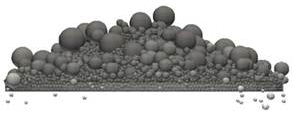
\includegraphics[width=.50\columnwidth]{images/065aorsim}
\caption[AoR sim]{Angle of repose simulation.}
\label{fig:065aorsim}
\end{figure}

\section{Shear Cell}
\label{sec:scsimulation}
%************************************************

\begin{figure}[!htb]
\centering
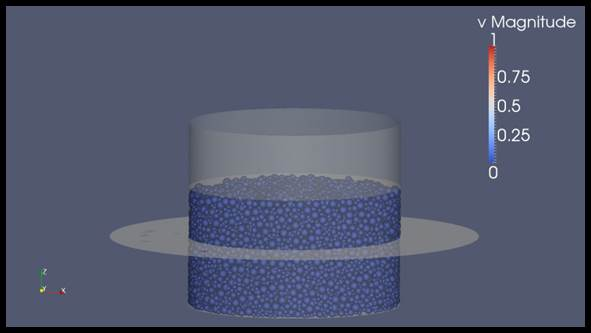
\includegraphics[width=.80\columnwidth]{images/007shearcellsim}
\caption[Shear cell simulation]{Shear cell simulation. The experimental device
was meticolously reproduced.}
\label{fig:007shearcellsim}
\end{figure}
\acs{LIGGGHTS}, the simulation toolbox we used, meets all the requirements of
modelling the shear tester described in \ref{sec:jsct}. 
First, it is capable of importing triangulated meshes of the two rings and a top lid. 
Since the real setup had a wall thickness, contact forces acting on a mesh are summed and can be saved, 
and thus shear force calculation is available out of the box. 
Second, the code can move a mesh with constant 
velocity as required for the measurement. 
To determine the shear stresses, the bulk solid had to be stressed with 
user-defined normal stresses. 
Therefore, a stress-controlled wall (servo-wall in \acs{LIGGGHTS}) was applied to the lid. \\
Although the geometry differs, the \acs{SCT} was designed to obtain the same values for the shear stresses as the 
Jenike shear cell tester (\acs{JSCT}), but with improved automation and reliability,
see Schulze \cite{RefWorks:118}. 
For this reason, the simulation setup was
based on the \acs{JSCT}, see Fig. \ref{fig:007shearcellsim}.
As suggested by Aigner et al. \cite{RefWorks:139} and Benvenuti et al. \cite{RefWorks:173}, 
the diameter and the height of the rings operated in the simulations had to be sufficiently large to avoid relevant wall effects. 
However, a larger domain increases the number of particles and thus
simulation time.
For this reason, we considered the cylinder dimension (\acs{dCylDp}), which is
proportional to the mean particle diameter, as an additional \acs{DEM}
parameter to be investigated. \\
A simulation run comprised four phases. 
First, the shear cell was filled with the granulate material, and it was allowed
to settle.
Then, the top lid was lowered and the first normal stress applied to the bulk
solid.
As in the experiment, the servo-wall allows calculating the position of the lid
while the first particle is being touched. 
The distance between the lid and the bottom of the domain multiplied by the 
simulation area gave the total volume.
Since the software already provided the total mass, we were able to calculate:
%************************************************
\begin{equation}
\rho_b = \frac{mass}{volume}.
 \label{eq:rhob}
\end{equation}

%************************************************
Next, the ring moved by a distance $l=0.1875 \cdot radius ~of ~the ~ring$, and
the required pre-shear force was measured.
Finally, the normal load was reduced to a fraction of the initial load, 
the ring was moved again by a distance $l$, and the shear force was recorded. 
Unlike in the original experiment, the bottom ring was moved to facilitate the numerical simulation. 
The velocity of the ring displacement, and consequently the total simulation time, 
was determined by a trade-off between minimizing the normal load oscillation and
optimizing computation time. 
The former requires (relatively) low velocity, and the latter requires high
speed.
We chose a constant velocity of $3*(mean ~ particle ~ radius)/seconds$, as the
best trade-off.\\
The normal stresses (pre-shear and shear phases) applied in each simulation were
the same as in the experiments.
The corresponding $\tau_{psh}$ and $\tau_{sh}$ were calculated - as in the experiments - from the mean of the plateau.\\
The input \acs{DEM} coefficients, \acs{CoR}, \acs{mus}, \acs{mur},
\acs{rhop} and \acs{dCylDp} (the cylinder dimension, proportional to the mean
particle diameter), as indicated in Table \ref{tab:10DEMVariableinputvalues}, 
were constant in each simulation, but their combination differed between
simulations.
Further, \acs{dCylDp} was used to evaluate the wall effect, but only $~10\%$ of the
simulations had a \acs{dCylDp} larger than $20$.
The normal stress \acs{sigman} and its
percentage during the incipient flow condition \acs{tauperc}
varied to replicate twelve shear-cell load conditions.\\ 
\begin{figure}[!htb] 
\centering 
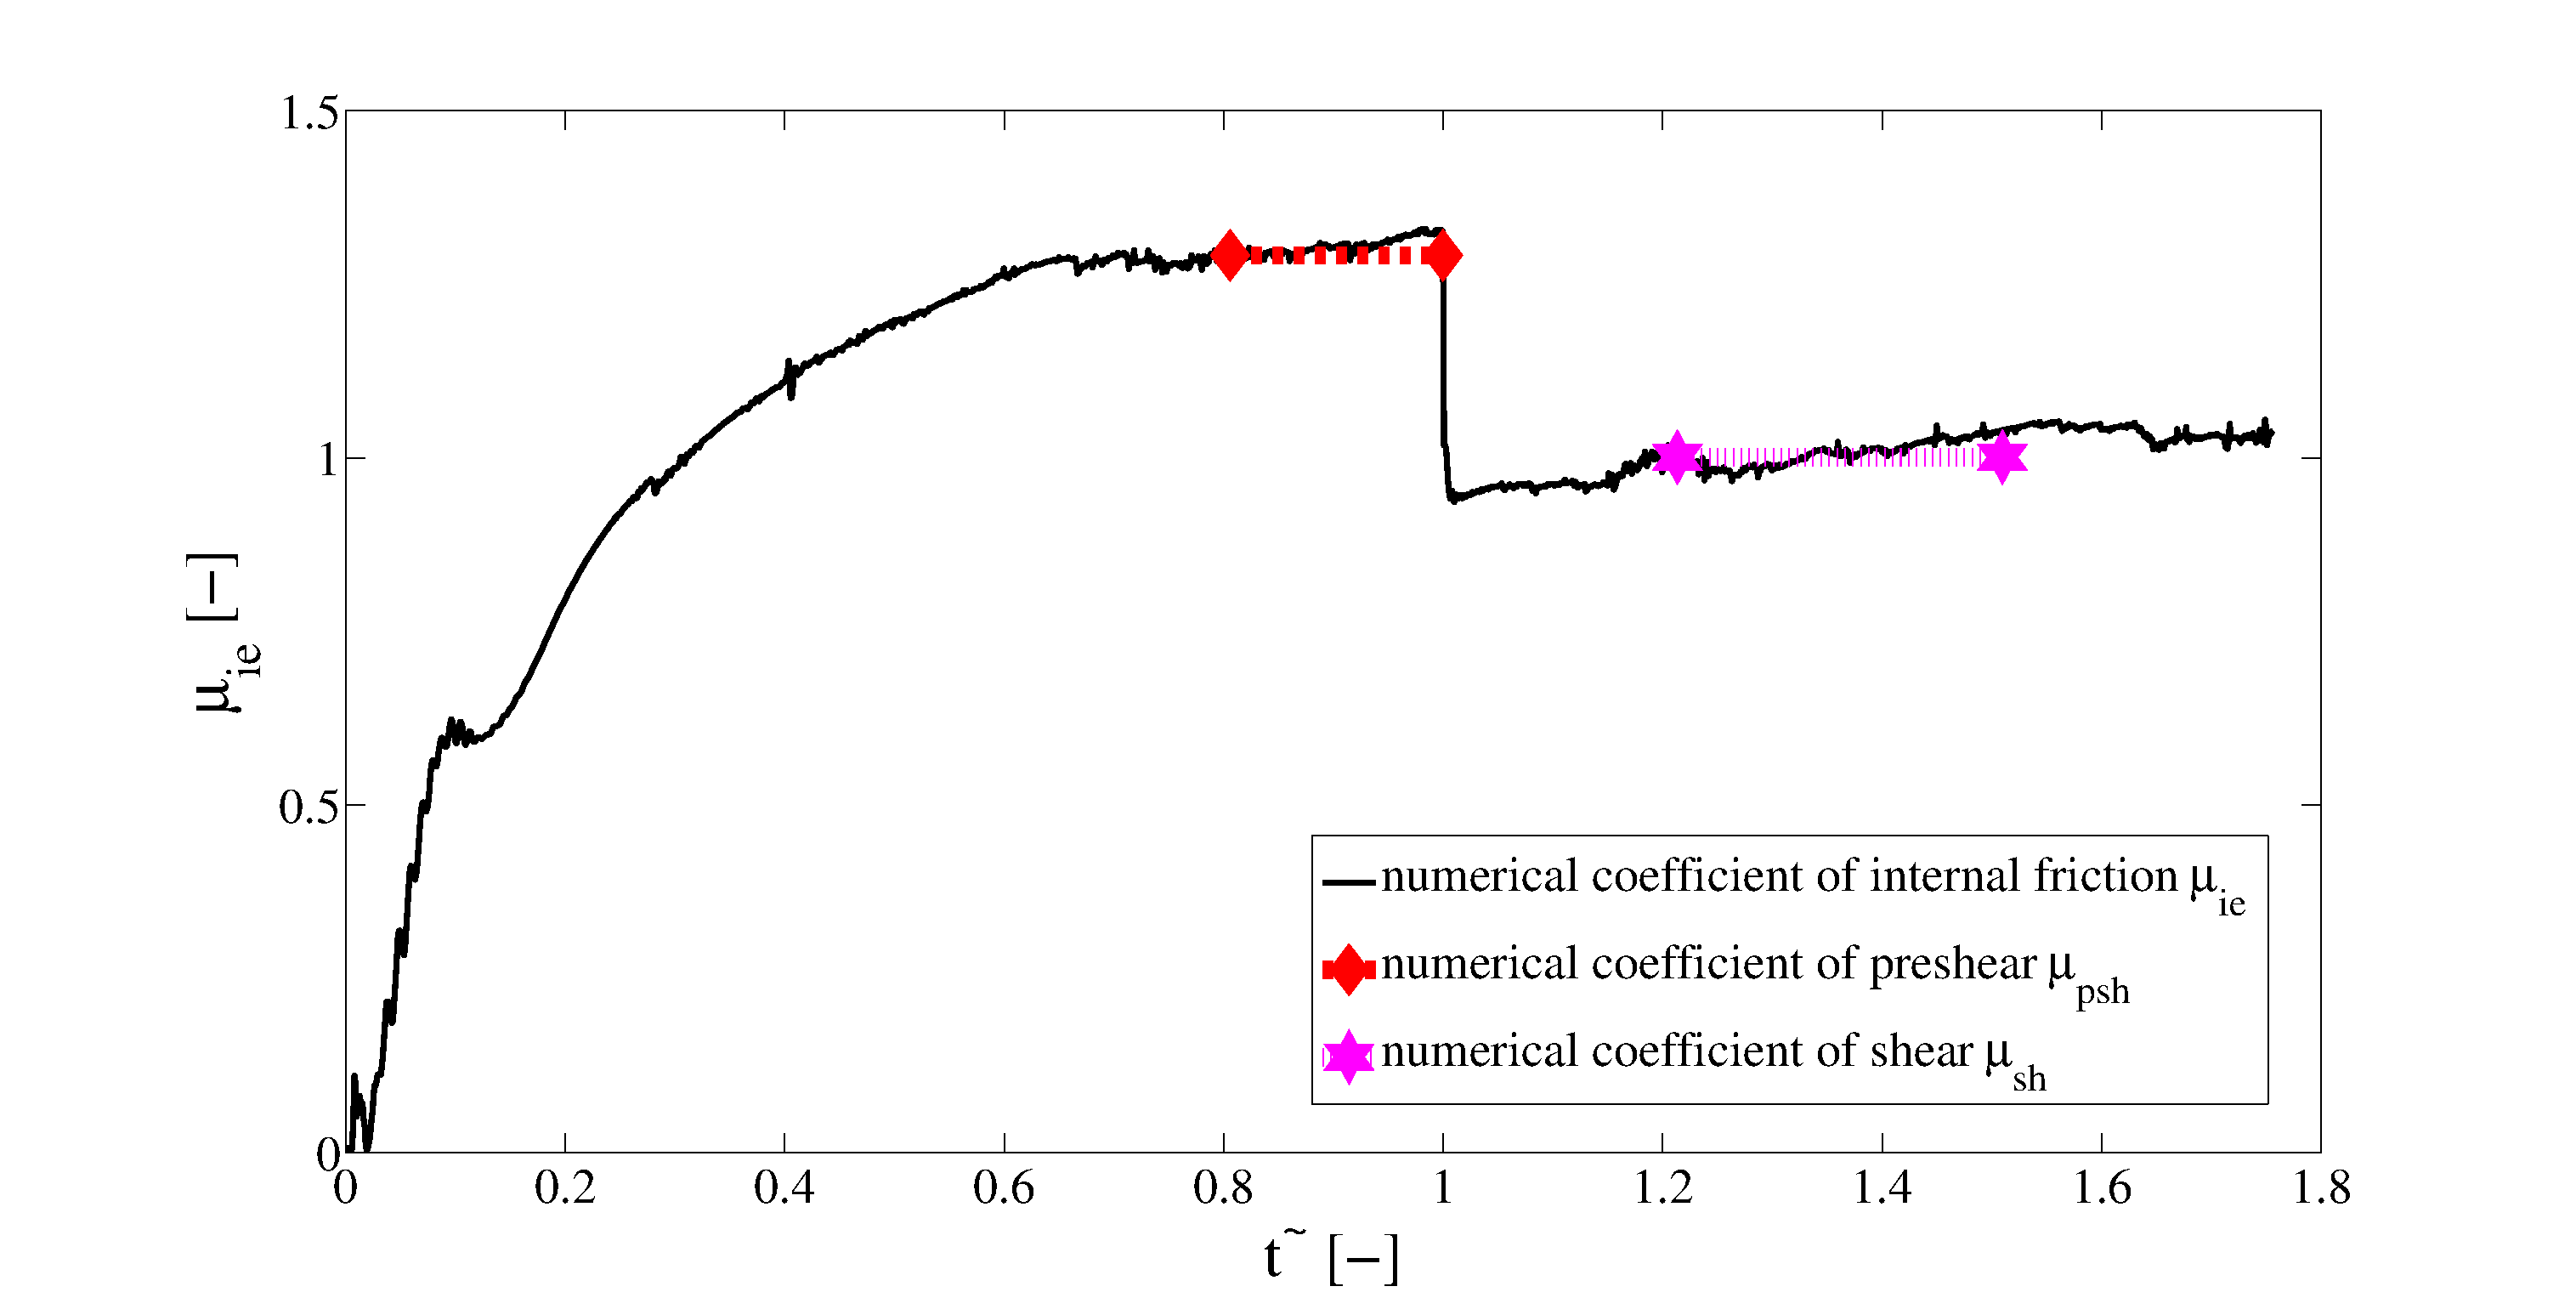
\includegraphics[width=.96\textwidth]{images/021simexample} 
\caption[Numerical shear cell tester stress path]{Numerical shear-cell tester
stress path - $\sigma_n = 10000 ~Pa$.}
\label{fig:021simexample} 
\end{figure}

% \begin{figure}[htp] \centering
%     \begin{subfigure}[b]{0.96\columnwidth}
%         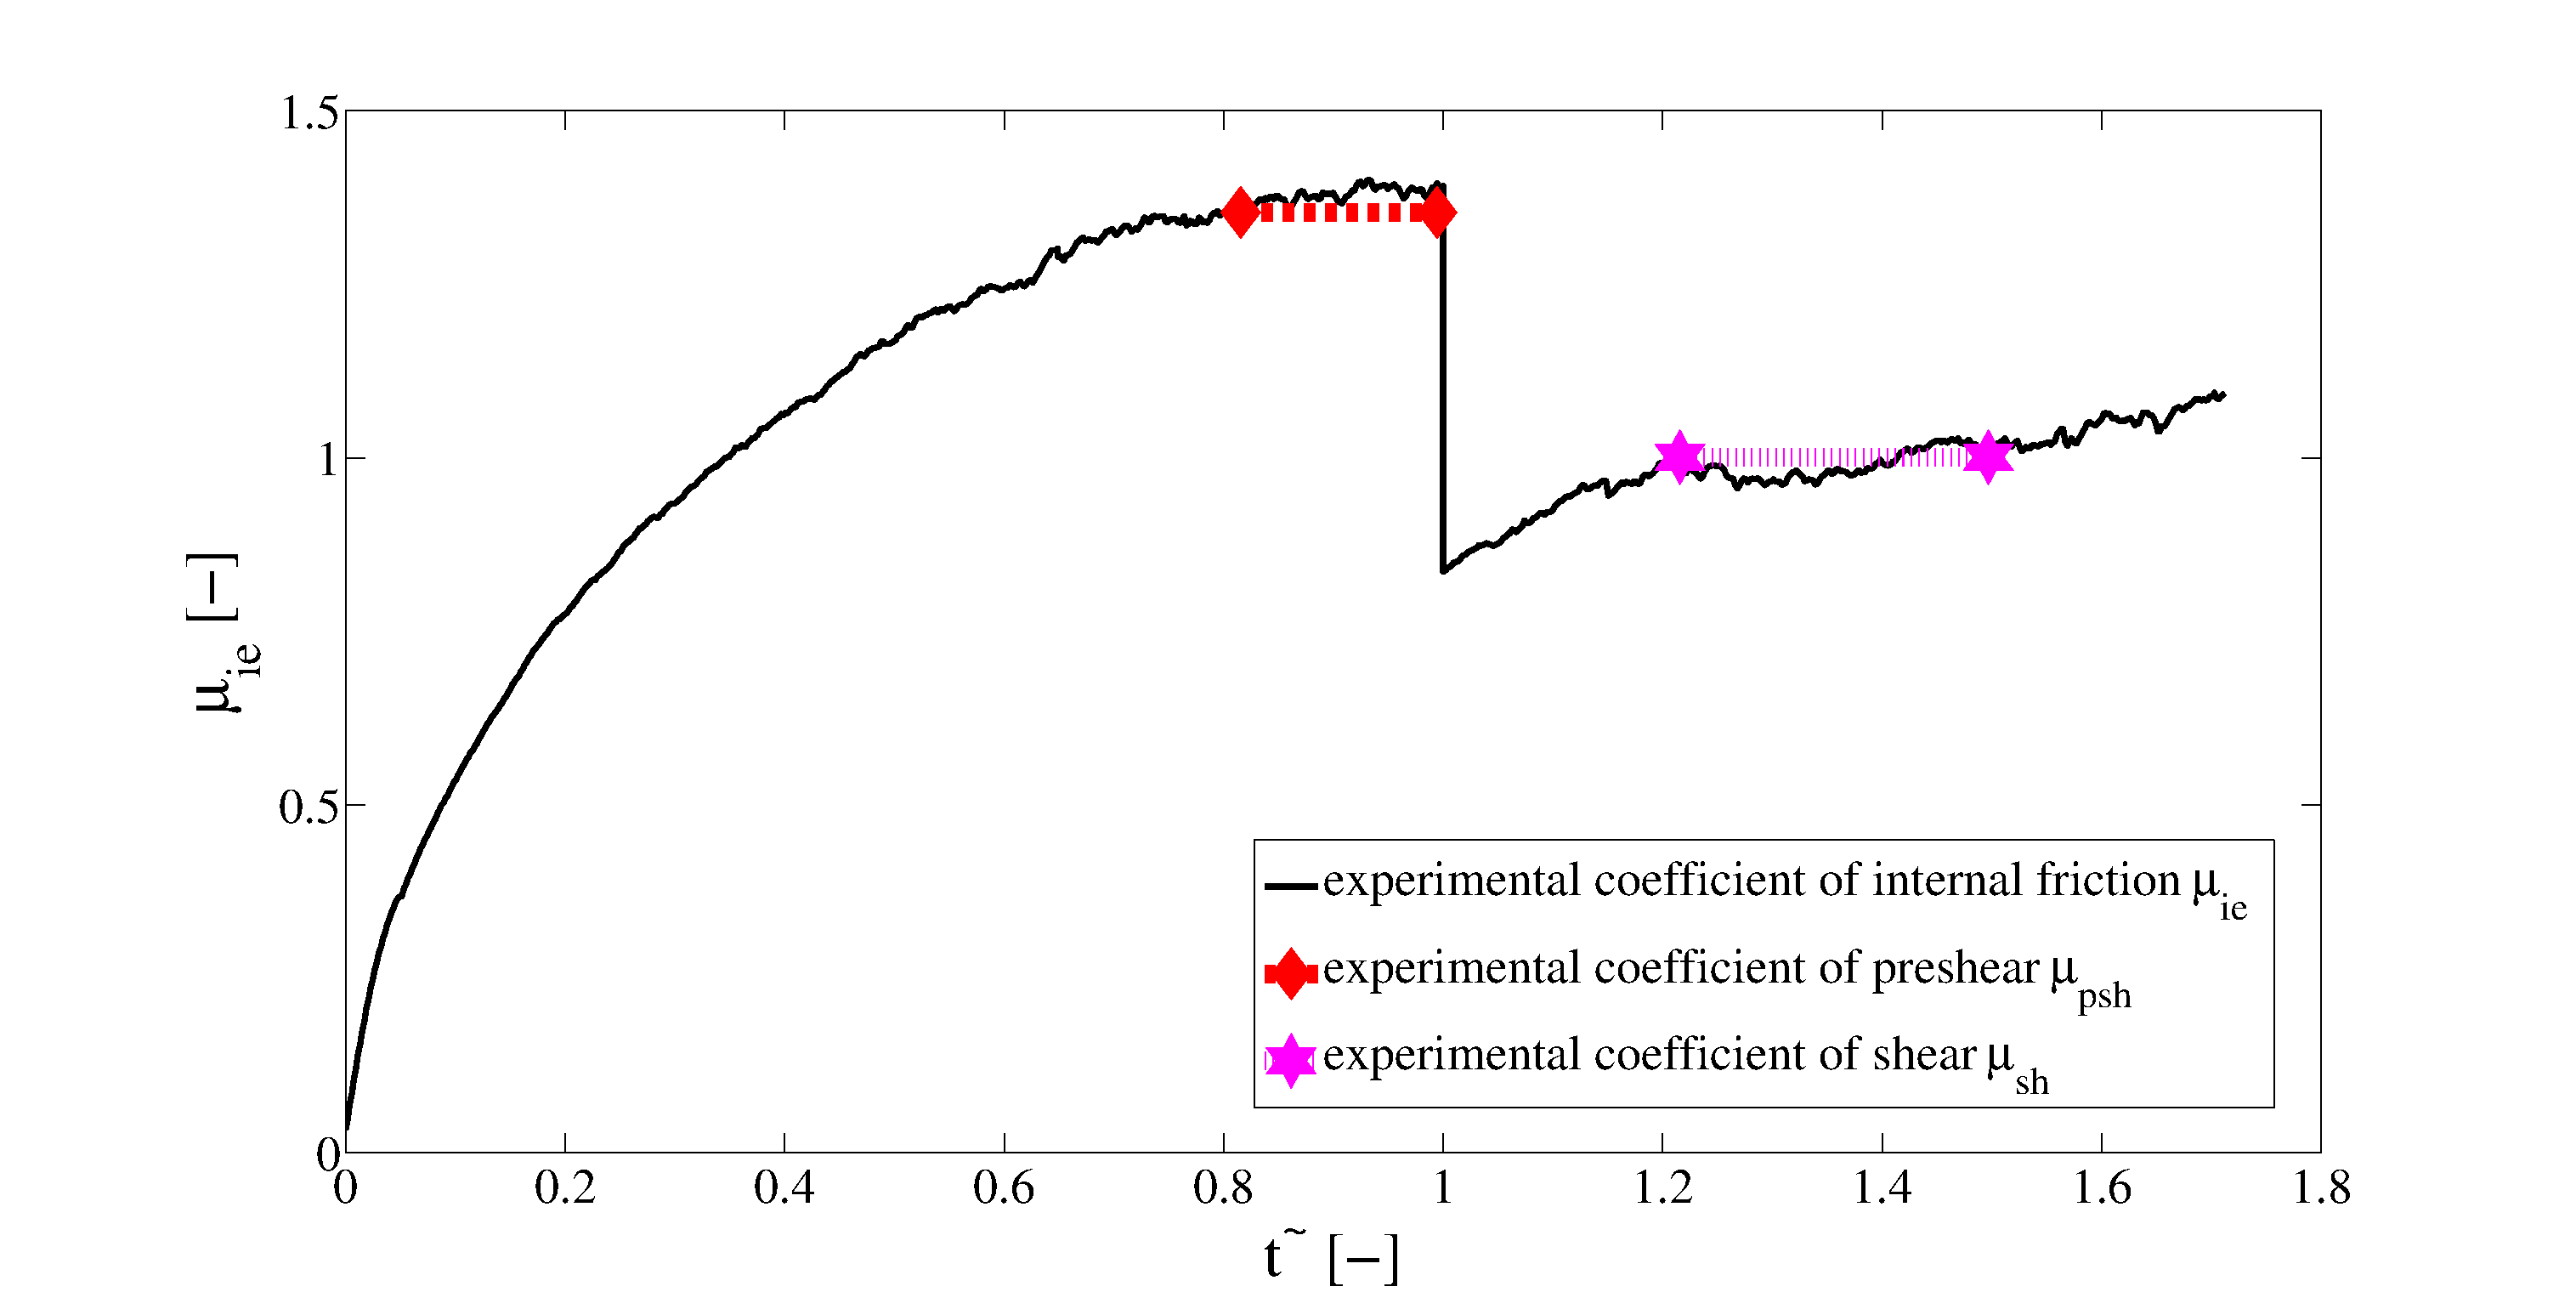
\includegraphics[width=\textwidth]{20experimental}
%         \caption{Experimental shear-cell tester stress path - $\sigma_n = 10000
%         ~Pa$}
%         \label{fig:20experimental} 
%     \end{subfigure}\\
%         \begin{subfigure}[b]{0.96\columnwidth}
%         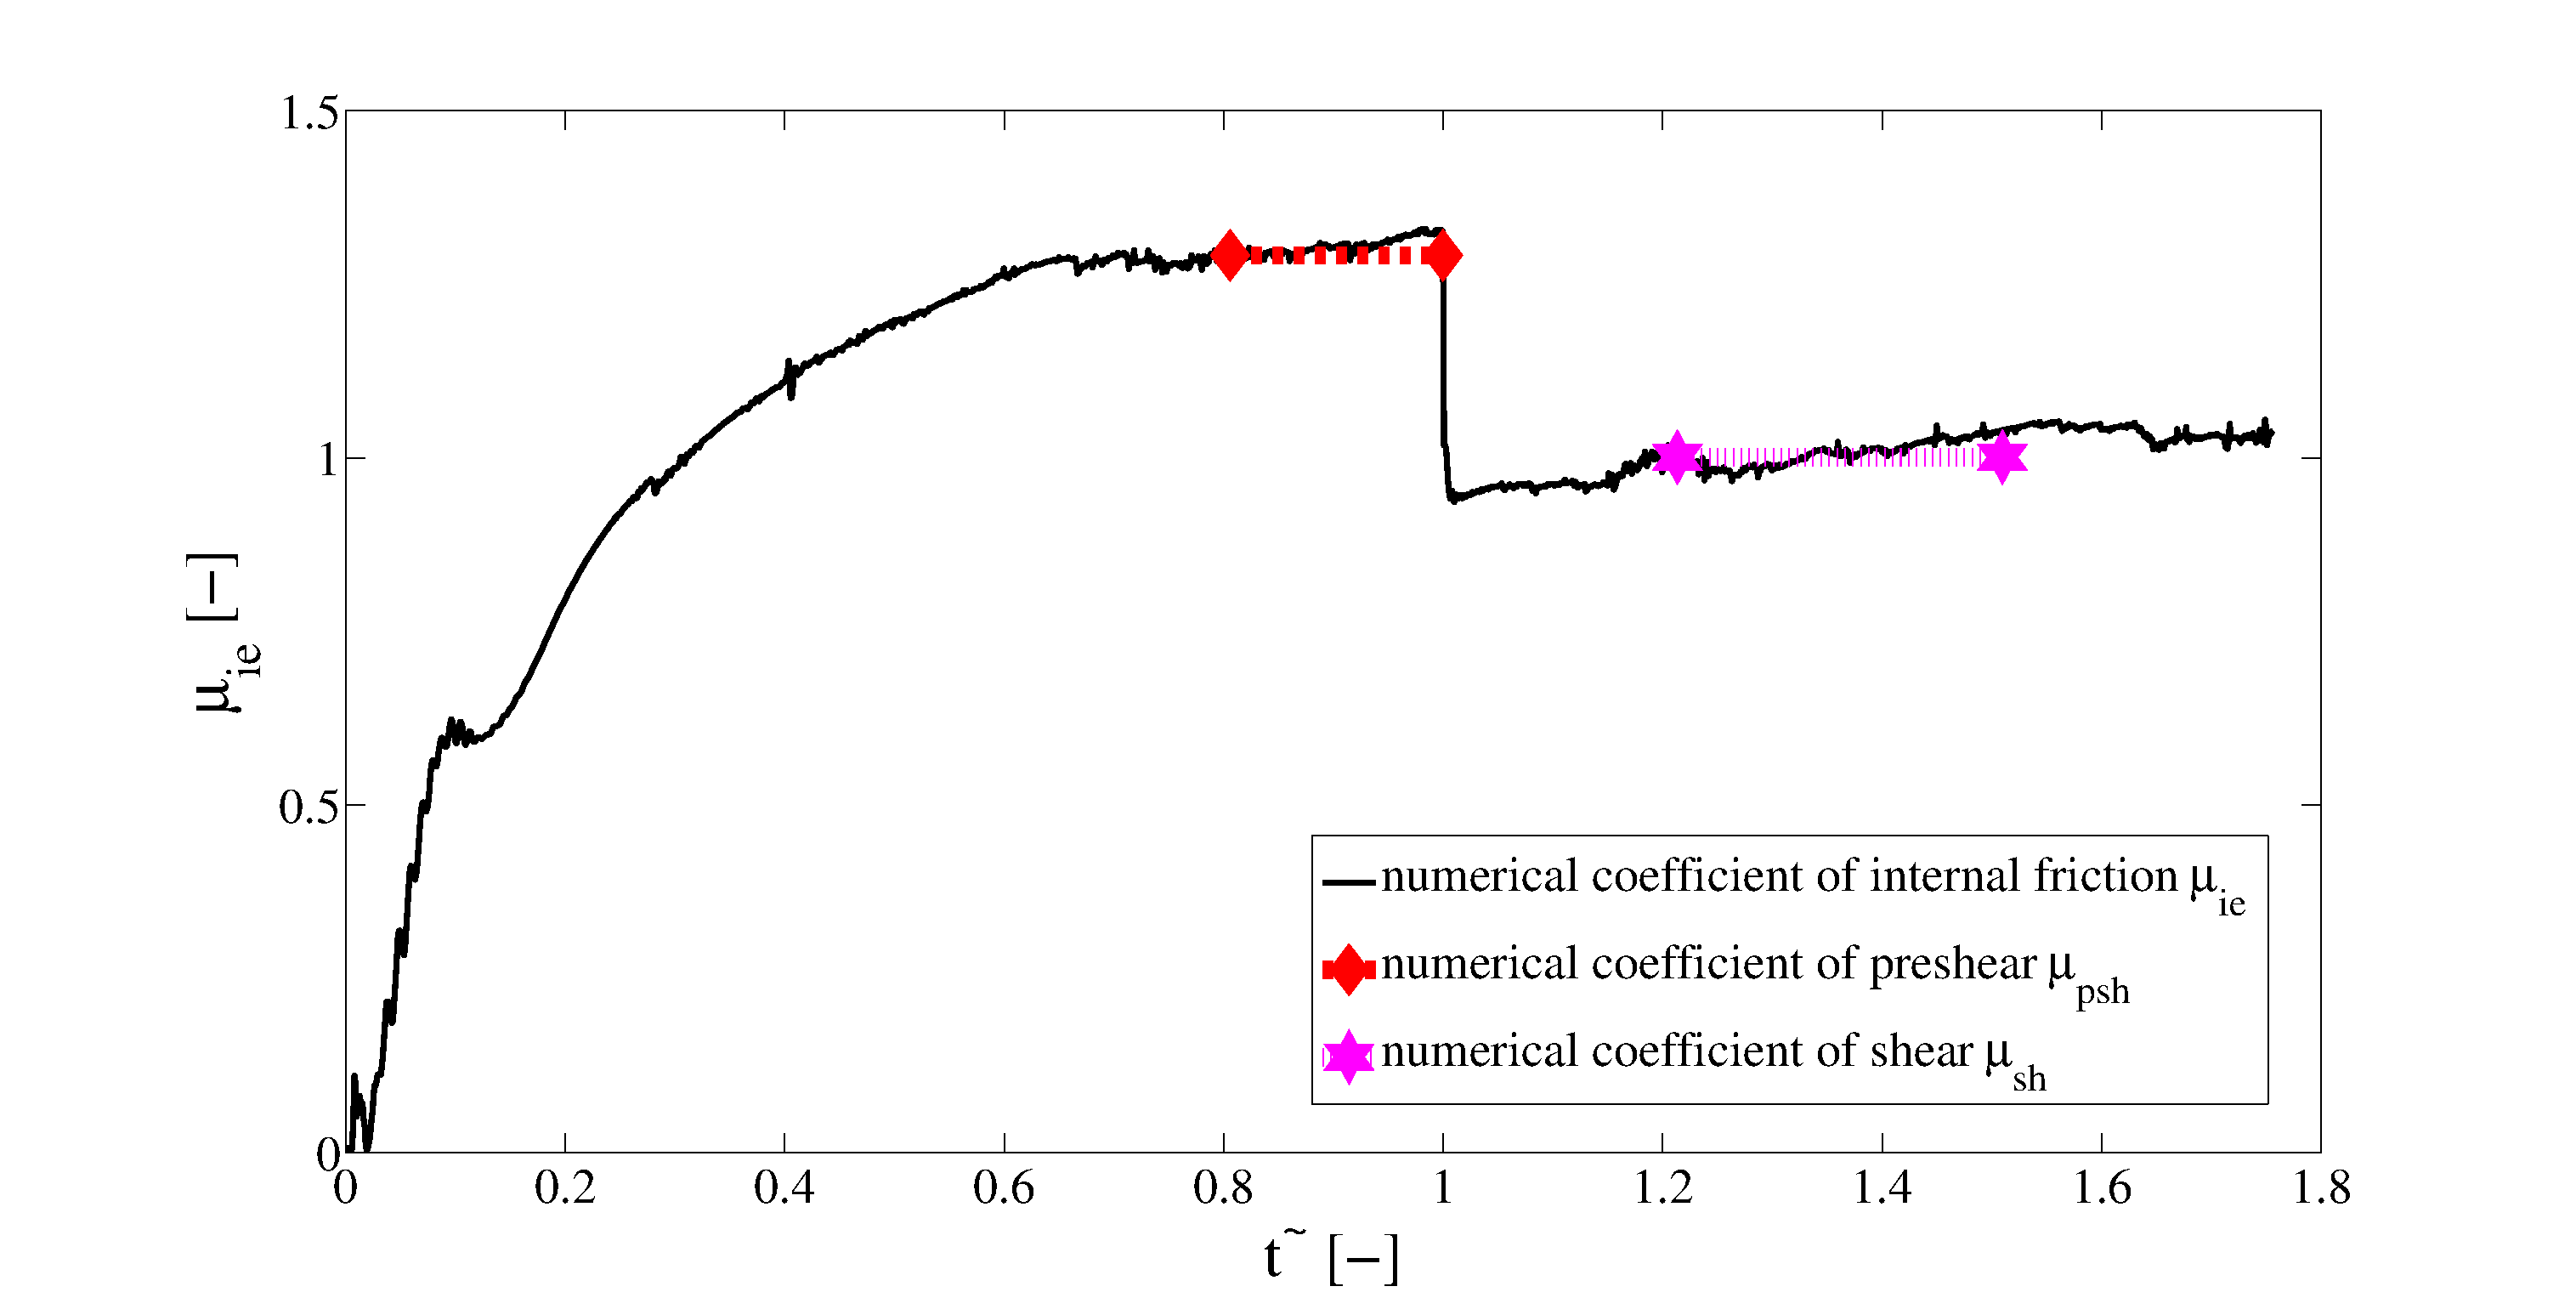
\includegraphics[width=\textwidth]{21simexample}
%         \caption{Numerical shear-cell tester stress path - $\sigma_n = 10000
%         ~Pa$}
%         \label{fig:21simexample} 
%     \end{subfigure}
%     \caption[Stress path]{Experimental and numerical samples of the stress path
%     for the Schulze ring shear cell tester.
% 	Time was normalized: $\tilde{t} = t/t_{change}$, where $t_{change}$ is the
% 	point in time at which the normal stress ($\sigma_n$) was modified during the
% 	tests.
% 	Until $\tilde{t}=1$, the $\sigma_n$ was kept constant at 10,000 Pa. 
% 	In Fig. \ref{fig:20experimental}, 
%  	a plateau was reached at $\tilde{t}~=0.91$.
% 	The coefficient of pre-shear (\ac{mupsh}) was calculated as the average of the
% 	coefficient of internal friction ($\mu_{ie}$) in this first plateau.
% 	At $\tilde{t}=1$, the $\sigma_n$ was reduced to $80 \%$ of its initial
% 	value, and soon after
% 	a second plateau developed.
% 	We obtained the coefficient of
% 	shear ($ \mu_{sh}$) as the average of $\mu_{ie}$ in this second plateau.
% 	The stress paths agree well, especially the plateaux.
% 	They were clearly relevant because
% 	the values representative of the bulk behaviours 
% 	were collected there.}
%     \label{fig:40experimentalsimulation}
% \end{figure}
Each \acs{SCT} simulation gave three of the \texit{bulk values} indicated in
Table \ref{tab:14bulkvalues}.
The first bulk value (\acs{rhob}) was provided directly. 
For correctly performed simulations, we
observed a stress path as in Fig. \ref{fig:021simexample}.
Time was normalized: $\tilde{t} = t/t_{change}$, where $t_{change}$ is the
point in time at which the normal stress (\acs{sigman}) was modified during the
tests.
Until $\tilde{t}=1$, the \acs{sigman} was kept constant at 10,000 Pa.
In Fig. \ref{fig:020experimental},
a plateau was reached at $\tilde{t}~=0.91$.
The coefficient of pre-shear (\acs{mupsh}) was calculated as the average of the
coefficient of internal friction (\acs{muie}) in this first plateau.
At $\tilde{t}=1$, the \acs{sigman} was reduced to $80 \%$ of its initial
value, and soon after
a second plateau developed.
We obtained the coefficient of
shear (\acs{mush}) as the average of \acs{muie} in this second plateau.
The stress paths agree well, especially the plateaux.
They were clearly relevant because
the values representative of the bulk behaviours
were collected there.\\
Together with the value from the \acs{AoR} simulation, we were able to define
the numerical bulk behaviour.


All the results in this chapter are pure \acs{DEM}, so they shoould be
materials agnostic, given the same particle distribution.

%*-*-*-*-*-%*-*-*-*-*-%*-*-*-*-*-%*-*-*-*-*-%*-*-*-*-*-%*-*-*-*-*-%*-*-*-*-*-%*-*-*-*-*-%*-*-*-*-*-
%*-*-*-*-*-%*-*-*-*-*-%*-*-*-*-*-%*-*-*-*-*-%*-*-*-*-*-%*-*-*-*-*-%*-*-*-*-*-%*-*-*-*-*-%*-*-*-*-*-

\section{Influence of variations of input parameters}
\label{sec:influence}

For sinter fine, 546 shear cell and 81 static \acs{AoR} simulations 
\wrong{write down all the simulations performed at the end.}
were run with
the parameter combinations described in Table
\ref{tab:10DEMVariableinputvalues}.
The computational time amounted to 1 hour with 32 AMD cores for a benchmark
shear-cell simulation and to 9 hours for a benchmark \acs{AoR} simulation, both with
50,000 particles.
Simulations with larger \acs{dCylDp} required more time (e.g., about 12 hours for
the shear cell with 400,000 particles ). \\

\begin{table}[h]
\centering
\begin{tabular}{ccccc}
\hline
    \acs{mus} & \acs{mur} & \acs{CoR} & \acs{rhop} & \acs{dCylDp} \\
    	$[-]$  & $[-]$   & $[-]$   & $[kg/m3]$ & $[-]$ \\
    \hline
    0.4 / 0.6 / 0.8 & 0.4 / 0.6 / 0.8 & 0.5 / 0.7 / 0.9 & 2500 / 3000 / 3500 & 20 / 36 / 38 / 40 \\

\hline
\end{tabular}
\caption[DEM variable input values]{DEM variable input values for training the
Neural Networks}
\label{tab:10DEMVariableinputvalues}
\end{table}.

\info{Some examples on how the numerical bulk values change when the DEM input
values change.}
\info{or sub-chapter with PCA?}

\section{PCA analysis}
\label{sec:pcaanalysis}

The linear relationship between the
training values can be seen in Table \ref{tab:06inputRelationshipTable}.
Sliding friction (\acs{mus}), rolling friction (\acs{mur}) and particle density (\acs{rhop})
had the greatest influence on, respectively, the coefficient of pre-shear
(\acs{mupsh}), the angle of repose  (\acs{AoR}) and the bulk density (\acs{rhob}). Notably, \acs{rhop}
was not used as a training parameter for \acs{AoR} bulk behaviour. 
\begin{table}[h]
\centering
\scalebox{1.0}{
\begin{tabular}{c|cccccccc}
\hline
          & $\mu_s$ & $\mu_r$ & $COR$ & $\rho_p$ & $\mu_{sh}$ & $\mu_{psh}$ & $\rho_{b}$ & $AOR$ \\
          \hline
    $\mu_s$ & 100.00 & 0.55  & 0.04  & 0.00  & 3.84  & 87.26 & 8.39  & 49.48 \\
    $\mu_r$ & 0.55  & 100.00 & 0.15  & 0.00  & 58.92 & 33.70 & 3.10  & 60.20 \\
    $COR$ & 0.04  & 0.15  & 100.00 & 0.00  & 15.52 & 0.57  & 1.71  & 0.00 \\
    $\rho_p$ & 0.00  & 0.00  & 0.00  & 100.00 & 4.98  & 5.71  & 99.00 & 0.00 \\
    $\mu_{sh}$ & 3.84  & 58.92 & 15.52 & 4.98  & 100.00 & 26.03 & 9.52  & 0.00 \\
    $\mu_{psh}$ & \textbf{87.26} & 33.70 & 0.57  & 5.71  & 26.03 & 100.00 & 4.33 
    & 0.00
    \\
    $\rho_{b}$ & 8.39  & 3.10  & 1.71  & \textbf{99.00} & 9.52  & 4.33  & 100.00
    & 0.00 \\
    $AOR$ & 49.48 & \textbf{60.20} & 0.00  & 0.00  & 0.00  & 0.00  & 0.00  &
    100.00 \\
    
\hline
\end{tabular}}
\caption{Values of linear relationship between considered variables multiplied
for 100}
\label{tab:06inputRelationshipTable}
\end{table}
\improvement{underline that is good that the input parameters are not
correlated}
